%% -*- coding: utf-8-unix -*-

\chapter{関連ソフトウェア}

 \section{Expectacle}
 \label{sec:expectacle}
 % tftp server – NetTester
 % \url{https://3.basecamp.com/3088280/buckets/867009/documents/268762822}
 % GitHub - stereocat/expectacle
 % \url{https://github.com/stereocat/expectacle/tree/develop}

テストシナリオ実装の際、テスト対象機器へのコマンド発行(teardown処理)をお
こなうためにExpectacle~\cite{expectacle}というツールを使用している。
Expectacle はあらかじめ作成したコマンド(列)を指定した機器情報に基づいて
順に送信する単純なツールである。詳細な使用方法についてはExpectacle
README にあるためここでは扱わない。本PoCで利用した際の注意事項について解
説する。

Expectacle が使用する操作対象機器情報・コマンド列ではERBを使った変数の展
開ができる。本PoCでは、操作対象情報のうちそのまま設定ファイルに記入して
リポジトリへ登録してはいけない秘密情報(ログインユーザ名・パスワード)を設
定するために環境変数展開を使用した。例として、L2/L3スイッチの操作に関し
ての操作対象情報は
\lstref{lst:l2sw1-login}\footnote{\url{https://github.com/net-tester/examples/blob/develop/features/support/expectacle/hosts/c3750g_hosts.yml}}
のようになる。
\begin{lstlisting}[caption=L2スイッチ(L2SW1)ログイン情報,label=lst:l2sw1-login]
- :hostname : 'l2sw1'
  :type : 'c3750g'
  :ipaddr : '192.168.20.150'
  :protocol : 'ssh'
  :username : "<%= ENV['L2SW_USER'] %>"
  :password : "<%= ENV['L2SW_PASS'] %>"
  :enable : "<%= ENV['L2SW_PASS'] %>"
\end{lstlisting}
\lstref{lst:l2sw1-login}ではログインユーザ名(\verb|L2SW_USER|)とパスワー
ド(\verb|L2SW_PASS|, ログイン/イネーブルが同一パスワード)を環境変数を参
照して設定している。そのため、テストシナリオ実行前に
\lstref{lst:l2sw1-login-envvar}のように環境変数を定義しておく。
\begin{lstlisting}[language=sh,caption=ログイン情報環境変数の設定,label=lst:l2sw1-login-envvar]
export L2SW_USER=username
export L2SW_PASS=password
\end{lstlisting}

環境変数によるパスワード等の設定は、そのままではコマンドヒストリ等に残っ
てしまうことがあるため、実行方法に注意が必要である\footnote{Expectacleで
は標準入力から環境変数の値を設定するスクリプトを同梱している:
\url{https://github.com/stereocat/expectacle/blob/develop/exe/readne}}。
Expectacleの機能は\tabref{tab:test-functions}の No.1 (NW機器の設定・操作)に
相当する。この機能は本プロジェクトの主要なスコープとしていないため、この
ような簡易な方法を採用している。

 \section{Debugging Trema}
 \label{sec:debugging-trema}
% 謎PacketInで死なずにログを出す – NetTester
% \url{https://3.basecamp.com/3088280/buckets/867009/todos/221324759}
% - Tremaのエラーログを出す – NetTester
%   \url{https://3.basecamp.com/3088280/buckets/867009/todos/210777914}
% - 今日なにした? – NetTester
%   \url{https://3.basecamp.com/3088280/buckets/867009/questions/181826801/answers/2016-09-08#__recording_221236017}

本プロジェクトの実行にあたって発生したOpenFlow関連の問題についての対処方
法(Tips)をまとめる。

  \subsection{Trema.logger}
  \label{sec:trema-logger}

当初、NetTester OFCのテーブルミスアクションを\code{CONTROLLER}として
packet-inを発生させるようにしていた。このとき、特定パケット(フレーム)の
packet-inに対して OFC (Trema) がエラーで停止しまうという問題が発生した
(\ref{sec:flow-priority-design}節参照)。この問題にあたって、Trema開発チー
ムの協力により、Tremaの内部ログを取得するための、\code{Trema.logger} API
が追加されている~\cite{trema-logger-doc}。

\code{Trema.logger}の使用方法は一般的なロガーと同様であり、Trema内部にロ
グメッセージを挿入していくことで、Tremaの内部情報のログを取得することが
できる。たとえば使用例は\lstref{lst:trema-logger-example}のようになる。
\begin{lstlisting}[caption=\code{Trema.logger}使用例,label=lst:trema-logger-example]
# lib/trema/switch.rb
def expect_receiving(expected_message_klass)
  loop do
    message = read
    # コントローラが受け取った OpenFlow メッセージをデバッグプリント
    Trema.logger.debug "Received an OpenFlow message: #{message.inspect}"
\end{lstlisting}

出力先のログファイルは \code{[ログディレクトリ]/trema.log} とな
る。\code{Trema.logger}を実行し内部ログを取得する場合、次のように実行時
ログレベルを指定する必要がある。
\begin{lstlisting}
trema run -l debug <controller>.rb
\end{lstlisting}
または verbose オプションを指定する(ログレベルは debug になる)。
\begin{lstlisting}
trema -v run <controller>.rb
\end{lstlisting}

  \subsection{Packet-in Binary Analysis}
  \label{sec:trema-packet-in-analysis}

\label{sec:trema-logger}節の事例(特定packet-inによるOFCの停止)については、
実際にpacket-inするバイナリを解析し、原因がTrema/Pio~\cite{pio}パケット
パーサのバグであることを突き止めた。ここではその際のデバッグ方法を記載す
る。

    \paragraph{OFCパケットキャプチャ}
そもそもTremaがどういったタイミング・原因で停止するのかを調査するために、
OFS-OFC間でやりとりされるOpenFlowメッセージのパケットキャプチャをとり、
OFC停止タイミングとの突合せをおこなっている。これによって、あるパケット
(フレーム)のpacket-inのタイミングでOFC停止が発生しているという仮説をたて
た。

    \paragraph{\code{Trema.logger}によるpacket-inのダンプ}
Trema内部の問題を取得するために、\label{sec:trema-logger}節に示した
\code{Trema.logger}を追加して、コントローラ停止時に処理しようとしていた
packet-inのダンプを取得する(\lstref{lst:packet-in-dump})。
\begin{lstlisting}[language=,caption=問題となるPacket-inの取得,label=lst:packet-in-dump]
diff --git a/lib/trema/switch.rb b/lib/trema/switch.rb
index 5a73005..d8c222e 100644
--- a/lib/trema/switch.rb
+++ b/lib/trema/switch.rb
@@ -34,7 +34,9 @@ module Trema
     end

     def read
-      OpenFlow.read read_openflow_binary
+      openflow_binary = read_openflow_binary
+      Trema.logger.debug openflow_binary.unpack('C*').inspect
+      OpenFlow.read openflow_binary
     end

     private
\end{lstlisting}

これにより、\lstref{lst:packet-in-log}のようにpacket-inダンプが取得できた。
\begin{lstlisting}[language=,caption=得られたPacket-in dump,label=lst:packet-in-log]
 D, [2016-09-14T11:29:41.312256 #21392] DEBUG -- : [1, 10, 0, 146, 0, 0, 0, 0, 0, 0, 1, 24, 1, 216, 0, 4, 0, 0, 1, 0, 12, 204, 204, 204, 0, 30, 73, 27, 157, 7, 1, 202, 170, 170, 3, 0, 0, 12, 32, 0, 2, 180, 19, 106, 0, 1, 0, 25, 76, 49, 80, 74, 95, 76, 50, 83, 87, 49, 46, 108, 49, 112, 106, 46, 108, 111, 99, 97, 108, 0, 5, 0, 251, 67, 105, 115, 99, 111, 32, 73, 79, 83, 32, 83, 111, 102, 116, 119, 97, 114, 101, 44, 32, 67, 51, 55, 53, 48, 32, 83, 111, 102, 116, 119, 97, 114, 101, 32, 40, 67, 51, 55, 53, 48, 45, 73, 80, 83, 69, 82, 86, 73, 67, 69, 83, 75, 57, 45, 77, 41, 44, 32, 86, 101, 114, 115, 105, 111, 110, 32, 49, 50, 46, 50, 40, 53]
D, [2016-09-14T11:29:41.313604 #21392] DEBUG -- : in Controller#start_switch_main(dpid=0x1), rescue (and unregister switch). error class:IOError, message:data truncated
\end{lstlisting}

    \paragraph{BinDataによる解析}
\lstref{lst:packet-in-log}をBinData(Trema/PioはBinDataをベースに実装され
ている)でパースして原因を調査する。パースは\lstref{lst:bindata-parse}の
ように実行することができる。

\begin{lstlisting}[language=,caption=BinDataによるパース,label=lst:bindata-parse]
irb> BinData.trace_reading do
irb>   Pio::OpenFlow.read [1, 10, 0, 146, 0, 0, 0, 0, 0, 0, 1, 24, 1, 216, 0, 4, 0, 0, 1, 0, 12, 204, 204, 204, 0, 30, 73, 27, 157, 7, 1, 202, 170, 170, 3, 0, 0, 12, 32, 0, 2, 180, 19, 106, 0, 1, 0, 25, 76, 49, 80, 74, 95, 76, 50, 83, 87, 49, 46, 108, 49, 112, 106, 46, 108, 111, 99, 97, 108, 0, 5, 0, 251, 67, 105, 115, 99, 111, 32, 73, 79, 83, 32, 83, 111, 102, 116, 119, 97, 114, 101, 44, 32, 67, 51, 55, 53, 48, 32, 83, 111, 102, 116, 119, 97, 114, 101, 32, 40, 67, 51, 55, 53, 48, 45, 73, 80, 83, 69, 82, 86, 73, 67, 69, 83, 75, 57, 45, 77, 41, 44, 32, 86, 101, 114, 115, 105, 111, 110, 32, 49, 50, 46, 50, 40, 53].pack('C*')
irb> end
obj.ofp_version => 1
obj.message_type => 10
obj.message_length => 146
obj.transaction_id-internal-.xid => 0
obj.transaction_id => 0
obj.body => "\x00\x00\x01\x18\x01\xD8\x00\x..."
obj.ofp_version => 1
obj. => nil
obj.message_type => 10
obj. => nil
obj.message_length => 146
obj.transaction_id-internal-.xid => 0
obj.transaction_id => 0
obj.buffer_id => 280
obj.total_len => 472
obj.in_port => 4
obj.reason-internal-.reason => 0
obj.reason => :no_match
obj.padding => 0
IOError: data truncated
        from /home/yasuhito/play/net-tester/vendor/bundle/ruby/2.3.0/gems/bindata-2.1.0/lib/bindata/io.rb:83:in `readbytes'
        from /home/yasuhito/play/net-tester/vendor/bundle/ruby/2.3.0/gems/bindata-2.1.0/lib/bindata/string.rb:110:in `read_and_return_value'
        from /home/yasuhito/play/net-tester/vendor/bundle/ruby/2.3.0/gems/bindata-2.1.0/lib/bindata/base_primitive.rb:124:in `do_read'
        from /home/yasuhito/play/net-tester/vendor/bundle/ruby/2.3.0/gems/bindata-2.1.0/lib/bindata/trace.rb:58:in `do_read_with_hook'
        from /home/yasuhito/play/net-tester/vendor/bundle/ruby/2.3.0/gems/bindata-2.1.0/lib/bindata/struct.rb:131:in `block in do_read'
        from /home/yasuhito/play/net-tester/vendor/bundle/ruby/2.3.0/gems/bindata-2.1.0/lib/bindata/struct.rb:131:in `each'
\end{lstlisting}

ここから、packet-in メッセージの \verb|total_len| の値が不正だったことが判明した。
\begin{itemize}
 \item OpenFlow ヘッダの全体の長さ (\verb|message_length| = 146) は正しい。
 \item 一方で \verb|PacketIn| の \verb|total_len| (PacketIn データの長さ)が
       \footnote{原因詳細まで調査していない。} 471 となっている。
 \item Pio はデータの長さを \verb|total_len| から取得するので、471 バイ
       ト読もうとして失敗している。
\end{itemize}

OpenFlow仕様によると、データ長は\verb|total_len|ではなく
\verb|message_len|から取得するように記述があった\footnote{OpenFlow1.0
Spec\cite{of10spec} ``5.4.1 Packet-in Message''参照。}ことから、Pioの
\verb|PacketIn|を修正することで問題は解決した\cite{pio-pr320}。なお、修
正後にパースをすると\lstref{lst:bindata-parse-re}ようになる。

\begin{lstlisting}[language=,caption=Pio修正後の再確認,label=lst:bindata-parse-re]
irb> Pio::OpenFlow.read [1, 10, 0, ... , 40, 53].pack("C*")
=> #<PacketIn open_flow_version: 1, message_type: 10, message_length: 146, transaction_id: 0x0, buffer_id: 0x118, total_length: 128, in_port: 4, reason: :no_match, data: #<Pio::EthernetFrame destination_mac: "01:00:0c:cc:cc:cc", source_mac: "00:1e:49:1b:9d:07", ether_type: 0x01ca, rest: "\xAA\xAA\x03\x00\x00\f \x00\x02\xB4\x13j\x00\x01\x00\x19L1PJ_L2SW1.l1pj.local\x00\x05\x00\xFBCisco IOS Software, C3750 Software (C3750-IPSERVICESK9-M), Version 12.2(5">>
\end{lstlisting}

  \subsection{Trema送受信メッセージログ}

% send/receive message
% - 今日なにした? – NetTester
%   \url{https://3.basecamp.com/3088280/buckets/867009/questions/181826801/answers/2016-09-27#__recording_241560820}
% - 送受信メッセージログ – NetTester
%   \url{https://3.basecamp.com/3088280/buckets/867009/messages/241506055}

最新版のTrema~\cite{trema-pr433}では、\ref{sec:trema-logger}節・
\ref{sec:trema-packet-in-analysis}節で実施したデバッグ作業をもとに、OFC
が送受信したOpenFlowメッセージをログで取得できるようになっている。
\lstref{lst:trema-ofmessage-debugprint}のように\code{-v}(verbose)オプショ
ンを指定することで利用できる。(\ref{sec:trema-logger}節で解説したように
ログファイル(\code{trema.log})にも出力される。)
\begin{lstlisting}[language=,caption=OpenFlowメッセージのデバッグプリント,label=lst:trema-ofmessage-debugprint]
% bundle exec trema -v run ./lib/hello_trema.rb -c trema.conf
sudo ovs-vsctl add-br br0xabc
sudo /sbin/sysctl -w net.ipv6.conf.br0xabc.disable_ipv6=1 -q
sudo ovs-vsctl set bridge br0xabc protocols=OpenFlow10 other-config:datapath-id=0000000000000abc
sudo ovs-vsctl set-controller br0xabc tcp:127.0.0.1:6653 -- set controller br0xabc connection-mode=out-of-band
sudo ovs-vsctl set-fail-mode br0xabc secure
Trema started.
Sending #<Pio::OpenFlow10::Hello:0x000000011190a8 @format={:version=>1, :type=>0, :_length=>8, :transaction_id=>0}>
Received #<Pio::OpenFlow10::Hello:0x0000000132c750>
Sending #<Pio::OpenFlow10::Echo::Request:0x0000000131ccd8 @format={:version=>1, :type=>2, :_length=>8, :transaction_id=>0, :body=>""}>
Received #<Pio::OpenFlow10::Echo::Reply:0x000000012ea288>
Sending #<Pio::OpenFlow10::Features::Request:0x000000012c9560 @format={:version=>1, :type=>5, :_length=>8, :transaction_id=>0}>
Received #<Pio::OpenFlow10::Features::Reply:0x000000012943d8>
Hello 0xabc!
Received #<Pio::OpenFlow10::Echo::Request:0x000000012099b8 @format={:version=>1, :type=>2, :_length=>8, :transaction_id=>0, :body=>""}>
Sending #<Pio::OpenFlow10::Echo::Reply:0x000000011ef338 @format={:version=>1, :type=>3, :_length=>8, :transaction_id=>0, :body=>""}>
...
\end{lstlisting}

\section{Phut Basics}
\label{sec:phut_basics}

ここでは、NetTesterの内部実装およびNetTester自身のテストコードで使用され
ているコードを元に、仮想ノード/仮想ネットワーク操作の処理実装の基礎につ
いて解説する。NetTester内部では、Phut~\cite{phut}を使用してLinuxの仮想ネッ
トワーク機能を操作している。なお、記載内容は 2016年9月時点のものである。

\subsection{Phutによる仮想ノード/仮想ネットワーク操作の概要}

まず、Phutによる virtual link/host/switch の操作のながれを理解する。
\begin{itemize}
 \item vLink を生成する
 \item vHost/vSwitch を生成する
       \begin{itemize}
        \item PhutではvHost/vSwitch を生成するときに interface device
              (vLinkの端点) を指定するので、通常は先に vLink を生成こと
              になる。
       \end{itemize}
 \item vLink と vHost/vSwitch を接続してトポロジを組み立てる。
\end{itemize}

vLink/vHost/vSwitch のいずれも、インスタンスを使うときは \verb|#create|
method を使用する。(\verb|create| は \verb|new| +
\verb|run|, \verb|start| という形になっている。単純に \verb|new| するだ
けでは active/enable にならない。)

インスタンスを操作したい場合は、インスタンス名(\verb|name| attribute)で
\verb|find_by| する。
\begin{lstlisting}
instance = Phut::<class>.find_by('instance_name')
\end{lstlisting}

\subsection{vLink}

\verb|Phut::Link| で vLink をつくる。これにより、
\figref{fig:vlink-model}のような vLink が作成される。

\begin{figure}[h]
 \centering
 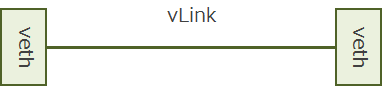
\includegraphics[scale=0.6]{img/phut-vlink-model.png}
 \caption{vLinkのモデル}
 \label{fig:vlink-model}
\end{figure}

これには「Phutで扱うための名前」と「OS上で使われる実際のデバイス名」があ
る。例えば、\verb|Phut::Link('sport', 'dport')|というコードに対しては、
\code{sport}, \code{dport}がPhutで扱うための名前となる。

Phutの内部処理で、Phutが識別するインタフェース名をもとに、OS上で使われる
実際のデバイス名(\code{L1\_sport}, \code{L1\_dport})が決められる
(\figref{fig:vlink-model2})。OS上(NetTester外)からPhutで生成したインスタ
ンスを操作する場合は、実際のデバイス名を使用する必要がある。また、デバイ
ス名として使用できる文字列には上限があるため、名前(文字列)の長さに注意す
る必要がある。

\begin{figure}[h]
 \centering
 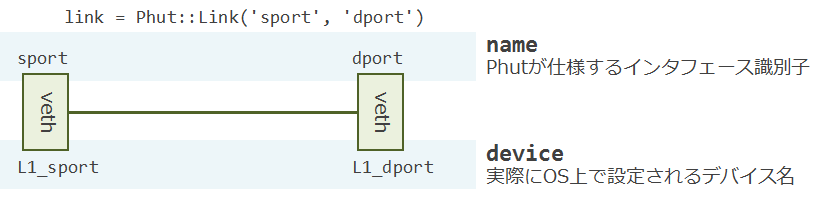
\includegraphics[scale=0.6]{img/phut-vlink-model2.png}
 \caption{インタフェースの名前とデバイス名}
 \label{fig:vlink-model2}
\end{figure}

生成した vLink(veth pair)をそのほかのインスタンス(vHost/vSwitch)に接続す
ることで仮想ネットワークを構成する。

\subsection{vHost}
Phutでは2種類のホストを取り扱う。

\paragraph{Phut::Vhost}

Rubyで実装された仮想ノードである。下記のように動作がシンプルで、直接的な
動作チェックに向いている。
\begin{itemize}
 \item UDPパケットの送受信ができる(\verb|#send_packet|)。
       \begin{itemize}
        \item ARPは送信せず、直接 IP(UDP) Unicastを送信する。
       \end{itemize}
 \item ARP処理しないので、あらかじめ ARP table を与えておく必要がある
       (\verb|arp_entries|で ``\verb|IP1/MAC1,IP2/MAC2,...|'' のような文
       字列を与える)。パケット送信(\verb|#send_packet|)するときに ARP
       entry が見つからなければ何もしない(パケットを送信しない)。
\begin{lstlisting}
arp_entries = "192.168.0.1/00:ba:dc:ab:1e:01,192.168.0.2/00:ba:dc:ab:1e:02"
\end{lstlisting}
\end{itemize}


インスタンスを作るときに、\verb|device| でこのホストに接続する veth を指
定する(\lstref{lst:create-vhost-instance})。
\begin{lstlisting}[caption=Phut::Vhostインスタンスの作成,label=lst:create-vhost-instance]
host = Phut::Vhost.create(name: 'host_name',
                          ip_address: ip_address,
                          mac_address: mac_address,
                          arp_entries: arp_entries,
                          device: link.device('interface_name'))
\end{lstlisting}

\paragraph{Phut::Netns}
Linux namespace で作成したホスト。何らかのコマンド(プロセス)を namespace
上で実行する形をとる。これは、ネットワークのみホストOSから分離した
(namespaceをわけた)状態で、OS上でコマンド実行するのと同様である。実行結
果の処理などは自分で作りこみをする必要があるが、その分自由度がおおきく、
OS上で実行可能な処理は原則そのまま利用できる。

Network Namespace は Linux OS の機能であるため、NetTesterで作成した
namespace であっても、NetTester の外側(OS)から使用可能である\footnote{OS
上で \code{sudo ip netns exec <host namespace> <command>} する。}。

複雑なデバッグ作業をやりたい場合は Netns を使う必要がある。インスタンス
を作ったあと \verb|#device=| でこのホストに接続する veth を指定する
(\lstref{lst:create-netns-instance})。

\begin{lstlisting}[caption=Phut::Netnsインスタンスの作成,label=lst:create-netns-instance]
host = Phut::Netns.create(name: 'host_name',
                          ip_address: ip_address,
                          netmask: '255.255.255.0',
                          mac_address: mac_address)
host.device = link.device('interface_name')
\end{lstlisting}

\subsection{vSwitch}

NetTester自体をテストするためのテストシナリオ
\footnote{\url{https://github.com/net-tester/net-tester/blob/develop/features/step_definitions/net_tester_physical_switch_steps.rb},
\url{https://github.com/net-tester/net-tester/blob/develop/features/step_definitions/net_tester_steps.rb}}
実装の中で、NetTester本体の起動では以下のような処理をしている
(\lstref{lst:run-nettester})。
\begin{lstlisting}[caption=NetTesterの起動,label=lst:run-nettester]
 Given(/^DPID が (\S+) の NetTester 物理スイッチ$/) do |dpid|
  @physical_test_switch = PhysicalTestSwitch.create(dpid: dpid.hex)
 end

 Given(/^NetTester を起動$/) do
  main_link = Phut::Link.create('ssw', 'psw')
  NetTester.run(network_device: main_link.device(:ssw),
                physical_switch_dpid: @physical_test_switch.dpid)
  @physical_test_switch.add_numbered_port(1, main_link.device(:psw))
 end
\end{lstlisting}

これにより、\figref{fig:phut-testee-switch}のように仮想ネットワークが構
成される。ここでは、NetTester自身のテストのために、物理スイッチに相当す
るものをvSwitch(ソフトウェアスイッチ, \verb|@physical_test_switch|)とし
て起動している。

\begin{figure}[h]
 \centering
 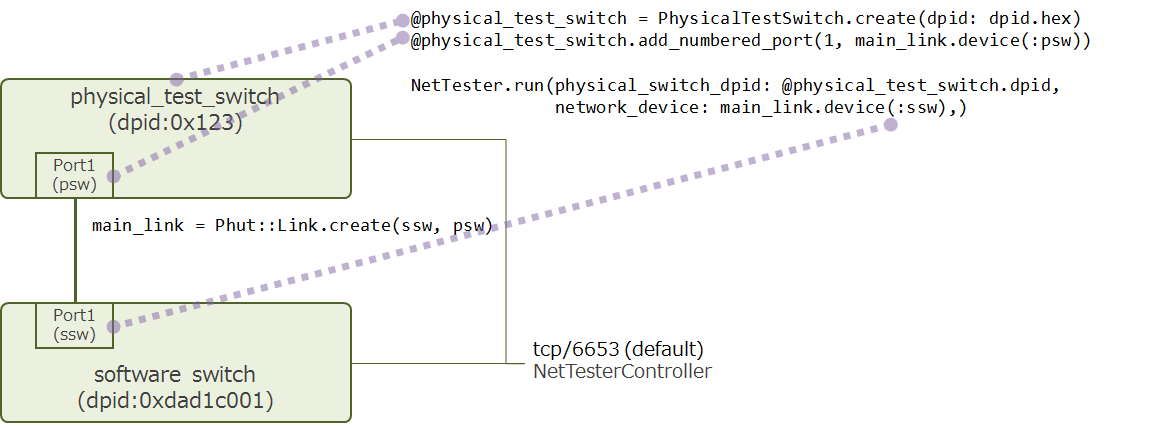
\includegraphics[scale=0.6]{img/phut-psw-ssw-model.png}
 \caption{テスト用物理スイッチ(相当)の起動と接続}
 \label{fig:phut-psw-ssw-model}
\end{figure}

\verb|NetTester.#run|の中では以下の処理をしている。

\begin{itemize}
 \item trema の起動 (NetTesterControllerの起動)
 \item ssw の起動
 \item ssw に veth (\verb|main_link.device(:ssw)|) を接続する。
       (port number 1)
\end{itemize}

\subsection{テスト対象としての vSwitch の利用}

NetTester 自身をテストする場合、テスト対象ネットワークに相当するものをテ
ストシナリオ中で用意する必要がある。テスト対象として vSwitch を起動する
場合は\lstref{lst:run-vswitch}のようにおこなう
\footnote{\url{https://github.com/net-tester/net-tester/blob/develop/features/step_definitions/ethernet_switch_steps.rb}}
。\lstref{lst:run-vswitch}では、テスト対象として使用する vSwitch の起動
およびコントローラとの接続(Learning Switchとして動作させるため)をおこなっ
ている。

\begin{lstlisting}[caption=vSwitchの起動,label=lst:run-vswitch]
Given(/^テスト対象のイーサネットスイッチ$/) do
  @testee_switch = TesteeSwitch.create(dpid: 0x1, tcp_port: 6654)
  step %(I successfully run `trema run ../../vendor/learning_switch/lib/learning_switch.rb --port 6654 -L #{Phut.log_dir} -P #{Phut.pid_dir} -S #{Phut.socket_dir} --daemon`)
end
\end{lstlisting}

テストシナリオ内部
\footnote{\url{https://github.com/net-tester/net-tester/blob/develop/features/step_definitions/net_tester_physical_switch_steps.rb}}
では、テスト対象ネットワーク(\verb|@testee_switch|)と物理スイッチ
(\verb|@physical_test_switch|)を接続するため、
\lstref{lst:connect-vswitch}のような処理をおこなう。

\begin{lstlisting}[caption=vSwitch間接続,label=lst:connect-vswitch]
Given(/^NetTester 物理スイッチとテスト対象のスイッチを次のように接続:$/) do |table|
  table.hashes.each do |each|
    pport_id = each['Physical Port'].to_i
    tport_id = each['Testee Port'].to_i
    port_name = "pport#{pport_id}"
    tport_name = "tport#{tport_id}"
    link = Phut::Link.create(tport_name, port_name)
    @physical_test_switch.add_numbered_port(pport_id, link.device(port_name))
    @testee_switch.add_numbered_port(tport_id, link.device(tport_name))
  end
end
\end{lstlisting}

これによって\figref{fig:phut-testee-switch}のように仮想ネットワークが構
成される。

\begin{figure}[h]
 \centering
 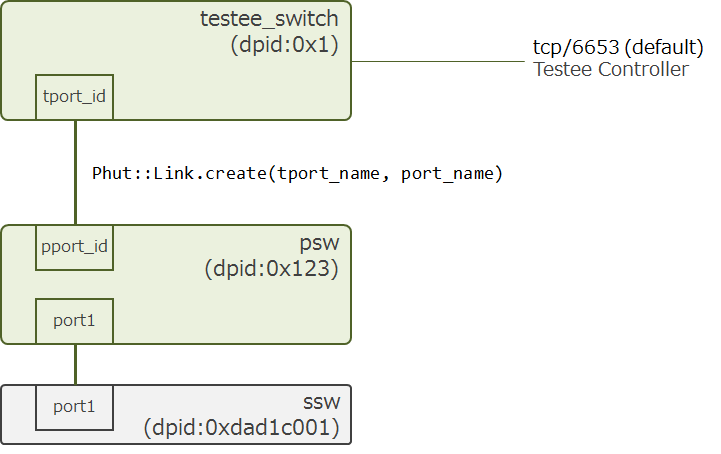
\includegraphics[scale=0.6]{img/phut-testee-switch.png}
 \caption{テスト対象機器(スイッチ)の生成と接続}
 \label{fig:phut-testee-switch}
\end{figure}

\subsection{テスト対象としての vHost の利用}

ポート間パッチのテスト
\footnote{\url{https://github.com/net-tester/net-tester/blob/develop/features/internal_tests/p2p_patch.feature}}
では、テスト対象ネッNetTesterのテストシナリオネットワークに属するノード
の生成・操作は\lstref{lst:create-testnode}のように記述している。

\begin{lstlisting}[caption=テスト用ノードの生成,label=lst:create-testnode]
  Background:
    Given DPID が 0x123 の NetTester 物理スイッチ
    And NetTester を起動
    And NetTester 物理スイッチとテスト対象ホストを次のように接続:
      | Physical Port | Host |
      |             2 |    1 |
      |             3 |    2 |
      |             4 |    3 |
\end{lstlisting}

テストシナリオ内部
\footnote{\url{https://github.com/net-tester/net-tester/blob/develop/features/step_definitions/p2p_patch_steps.rb}}(\lstref{lst:operate-testnode})
では、テストシナリオ(\lstref{lst:create-testnode})であたえられたテスト用
ノードのパラメタを元に以下のようにノードを生成し、テストを実行する。

\begin{lstlisting}[caption=テスト用ノードの生成と操作,label=lst:operate-testnode]
Given(/^NetTester 物理スイッチとテスト対象ホストを次のように接続:$/) do |table|
  ip_of_host = {}
  mac_of_host = {}
  vhost_arp_list = []

  table.hashes.each do |each|
    host_id = each['Host']
    ip_address = "192.168.0.#{host_id}"
    ip_of_host[host_id] = ip_address
    mac_address = "00:ba:dc:ab:1e:#{sprintf('%02x', host_id)}"
    mac_of_host[host_id] = mac_address
    vhost_arp_list.append "#{ip_address}/#{mac_address}"
  end

  arp_entries = vhost_arp_list.join(',')
  table.hashes.each do |each|
    pport_id = each['Physical Port'].to_i
    pport_name = "pport#{pport_id}"
    host_id = each['Host']
    host_name = "host#{host_id}"
    link = Phut::Link.create(host_name, pport_name)
    Phut::Vhost.create(name: host_name,
                       ip_address: ip_of_host[host_id],
                       mac_address: mac_of_host[host_id],
                       device: link.device(host_name),
                       arp_entries: arp_entries)
    @physical_test_switch.add_numbered_port(pport_id, link.device(pport_name))
  end
end
\end{lstlisting}

\lstref{lst:operate-testnode}では\verb|Phut::Vhost|を使用している。すべ
てのテスト用ノードの \verb|arp_entries| を作るために IP/MAC を用意すると
ころと、Phut instance を生成するパートに分割している。これにより、
\figref{fig:phut-testee-host}のように複数のテスト用ノードが作成され、テ
スト対象ネットワークとして物理スイッチ(\verb|psw|)に接続される。

\begin{figure}[h]
 \centering
 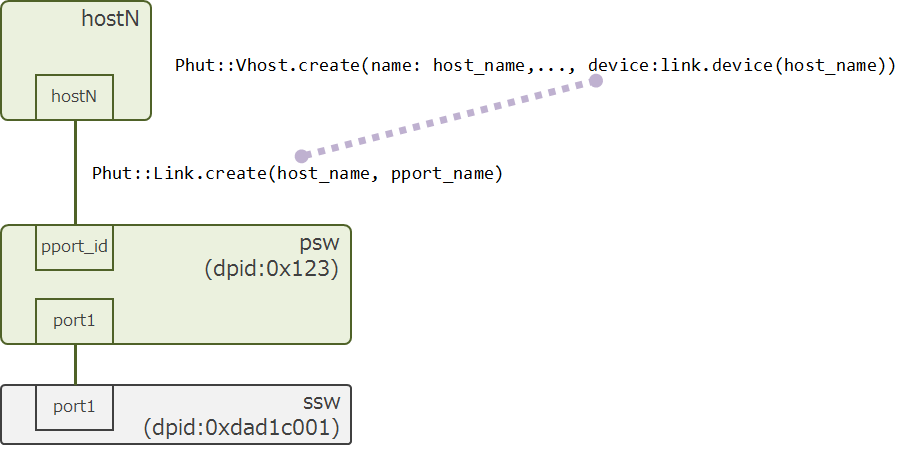
\includegraphics[scale=0.6]{img/phut-testee-host.png}
 \caption{テスト対象機器(ホスト)の生成と接続}
 \label{fig:phut-testee-host}
\end{figure}

%%% Local Variables:
%%% mode: yatex
%%% TeX-master: "main.tex"
%%% End:
